% Template for ICIP-2013 paper; to be used with:
%          spconf.sty  - ICASSP/ICIP LaTeX style file, and
%          IEEEbib.bst - IEEE bibliography style file.
% --------------------------------------------------------------------------
\documentclass{article}
\usepackage{spconf,amsmath,graphicx,amssymb}

% Example definitions.
% --------------------
\def\x{{\mathbf x}}
\def\L{{\cal L}}

\DeclareMathOperator*{\argmin}{argmin} % no space, limits underneath in displays
\DeclareMathOperator*{\argmax}{argmax}

% Title.
% ------
\title{Report: Pattern Recognition}
%
% Single address.
% ---------------
\name{Leif Van Holland}
\address{University of Bonn}
%
% For example:
% ------------
%\address{School\\
%	Department\\
%	Address}
%
% Two addresses (uncomment and modify for two-address case).
% ----------------------------------------------------------
%\twoauthors
%  {A. Author-one, B. Author-two\sthanks{Thanks to XYZ agency for funding.}}
%	{School A-B\\
%	Department A-B\\
%	Address A-B}
%  {C. Author-three, D. Author-four\sthanks{The fourth author performed the work
%	while at ...}}
%	{School C-D\\
%	Department C-D\\
%	Address C-D}
%
\begin{document}
%\ninept
%
\maketitle

\section{Introduction}
\label{sec:intro}

In the last decades, unprecedented amounts of data are collected in various places throughout the analog and digital world. The amount of information renders manual interpretation unfeasible if not impossible. Therefore the topic of \emph{pattern recognition} plays an increasingly important role in modern technology. \\
The university lecture "Pattern Recognition"... \\
In the following... in order of the projects

\section{Regression}
The term \emph{regression} refers to a statistical method of estimating relationships between variables. Given a set of data $D = \left\{ (x_i,y_i) \right\} _{i=1}^N$, where $x_i \in \mathbb{R}^N$ and $y_i \in \mathbb{R}$, the goal is to find a set of parameters $\theta \in \mathbb{R}^k$ of a given model $y:\mathbb{R}^N \times \mathbb{R}^k \to \mathbb{R}$, such that $y$ \emph{predicts} the values $y_i$ based on $x_i$ as an input with minimal error. In other words, we look for parameter values $\hat{\theta}$ such that
\begin{equation} \label{eq:argmin}
\hat{\theta} = \argmin_\theta E(\theta).
\end{equation}
$E$ denotes the \emph{objective function} that depends on the problem at hand. Most times however, $E$ measures a distance between the target output $y_i$ and the model prediction $y(x_i,\hat{\theta})$.
\subsection{Maximum Likelihood Estimation}
If we choose a probability distribution $N$ based on parameters $\theta$ as our model, i.e. we suspect our data to be realizations of random variables $X_i\sim N[\theta]$, we can calculate the probability of any possible realization $x_i$ of $X_i$ depending on $\theta$. Bayes' formula yields
\[ P(x_i|\theta) = \frac{P(\theta|x_i)P(x_i)}{P(\theta)}\]
and we define the \emph{likelihood} $L$ that parameters $\theta$ are responsible for generating the set of data $D$ as a a function
\[ L(\theta,D) := P(\theta|D) = \frac{P(D|\theta)P(\theta)}{P(D)}. \]
If we assume that the random variables $X_i$ are i.i.d., we can further simplify that definition and rewrite the joint density $P(D)$ as a product and thus get
\[ L(\theta,D) = \prod_{x_i\in D} P(\theta|x_i).\]
For numerical stability, one often considers the \emph{log-likelihood} function
\[ \mathcal{L}(\theta,D) = \text{ln }L(\theta,D) = \sum_{x_i\in D} \text{ln }P(\theta|x_i).\]
To find the parameters $\theta$ that are most likely to have generated $D$, we look for the \emph{maximum likelihood estimate}
\[\hat{\theta} = \argmax_\theta L(\theta, D) = \argmin_\theta - L(\theta,D) \]
\subsection{Normal and Weibull Distribution}
In the first project we looked at two distributions applied to 1-dimensional data.
The \textbf{1D normal distribution} is $N[\mu,\sigma^2]$ depending on two parameters $\mu,\sigma^2\in\mathbb{R}$ with the density function
\[f(x)=\frac{1}{\sqrt{2\pi \sigma^2}} e^{\frac{1}{2}(\frac{x-\mu}{\sigma})^2}.\]
Using the method of maximum likelihood estimation we can specify the optimal choice $\hat{\mu}$ and $\hat{\sigma}^2$ for both parameters of the normal distribution directly, which coincide with the \emph{sample mean} and \emph{population variance} of the given set of data respectively:
\[\hat{\mu} = \frac{1}{n}\sum_{i=1}^n x_i \:\text{ and }\: \hat{\sigma}^2 = \frac{1}{n}\sum_{i=1}^n (x_i - \hat{\mu})^2\]
The result of this estimation on the body sizes from the data introduced in \ref{sec:data-used} can be seen in figure \ref{fig:body-normal}.\\

\begin{figure}
\centering
  \centerline{\includegraphics[width=8.5cm]{img/project1/plot2}}
\caption{Resulting PDF of a normal distribution maximizing the likelihood w.r.t. the body sizes from the data set introduced in \ref{sec:data-used}.}
\label{fig:body-normal}
\end{figure}

The \textbf{Weibull distribution} on the other hand uses parameters $\kappa, \alpha\in \mathbb{R}$ and is defined by the density
\[f(x) = \frac{\kappa}{\alpha}\left(\frac{x}{\alpha}\right)^{\kappa-1}e^{-(\frac{x}{\alpha})^\kappa}.\]
Estimating the parameters here is more involved, as there is no closed-form solution for the estimates $\hat{\kappa}$ and $\hat{\alpha}$. A maximum of the log-likelihood function
\[L(\alpha,\kappa) = N(\log \kappa - \kappa \log \alpha) + (\kappa-1)\sum_i \log d_i - \sum_i \left(\frac{d_i}{\alpha}\right)^{\kappa}\]
has therefore to be found numerically and we used Newton's method initialized with $\kappa=1$ and $\alpha=1$. To optimize the calculation time we rewrote the log-likelihood using a histogram $h(x_j) = h_j$ for all occurring values $x_j$ in the data, which reduces the number of elements the sums in $L$ are iterating over. $L(\alpha,\kappa)$ then equals the term
\[N(\log \kappa - \kappa \log \alpha) + (\kappa-1)\sum_j x_j \log h_j - \sum_j \left(\frac{x_j\cdot h_j}{\alpha}\right)^{\kappa}\]
We used the described method on Google Trends data about global interest in the search term \emph{"myspace"}, measured every week between January 1, 2003 and March 16, 2012. Figure \ref{fig:myspace-weibull} shows that assuming a Weibull distribution reasonably describes the overall trend for the most part, although one can clearly observe a deviation from the actual graph between weeks 100 and 200.
\begin{figure}
\centering
  \centerline{\includegraphics[width=8.5cm]{img/project1/plot3}}
\caption{MLE-fitted PDF of a Weibull distribution on Google Trends data describing the evolution of global interest in the search term \emph{"myspace"}.}
\label{fig:myspace-weibull}
\end{figure}


\subsection{Least Squares Technique}
basic idea, normal equations, pseudoinverse, least squares as special case of MLE (under gaussian noise)
example: fractal dimensions, polynomials
\subsection{Bayesian Regression}
first conditional expectation, this leads to bayesian regression
\subsection{Boolean Functions}
example to use least squares, show how we can find a linear combination of the boolean basis to reconstruct the rules. In fact we increase the dimension of the problem to get better results.
\section{Classification}
basic idea of classification
\subsection{Nearest Neighbors}
short explanation of nn
\subsection{kD-Trees}
short explanation of kd trees
\subsection{k-Means Clustering}
different algorithms for k-means
\subsection{Spectral Clustering}
stuff about fiedler vector, spectral clustering from computer vision
\subsection{Dimensionality Reduction}
pca and lda, explanation of differences
\subsection{Non-Monotonous Neurons}

\subsection{support vector machines}
short explanation of kernel trick and its implementation
\section{numerical instabilities}
throughout the projects special care for numerical issues
\section{conclusion}



























\section{model fitting}
\label{sec:models}
Most of the problems considered in this report are based on a given set of data $D = \left\{ (x_i,y_i) \right\} _{i=1}^n$, where $x_i \in \mathbb{R}^n$ and $y_i \in \mathbb{R}$. The general goal is to find a set of parameters $\theta \in \mathbb{R}^k$ of a given model $y:\mathbb{R}^n \times \mathbb{R}^k \to \mathbb{R}$, such that $y$ \emph{predicts} the values $y_i$ based on $x_i$ as an input with minimal error. In other words, we look for parameter values $\hat{\theta}$ so that
\begin{equation} \label{eq:argmin}
\hat{\theta} = \argmin_\theta E(\theta)
\end{equation}
$E$ denotes the \emph{objective function} that depends on the problem at hand. Most times however, $E$ measures a distance between the target output $y_i$ and the model prediction $y(x_i,\hat{\theta})$.

\subsection{Least squares}
A common approach is to construct an overdetermined linear system of $m$ equations and $n$ variables $Ax=b$, where $A\in\mathbb{R}^{m\times n}$, $b\in\mathbb{R}^m$ are given and we are looking for the solution $x\in\mathbb{R}^n$. Since it is overdetermined, which implies $m\geq n$, there is no exact solution in general. We rather look for an $x$ that minimizes the (euclidean) length of the residual $r = b-Ax \in\mathbb{R}^m$, i.e.
\begin{equation} \label{eq:lstsq}
\lVert b-Ax \lVert_2 \: \rightarrow \min
\end{equation}
Minimizing the length of $r$ is equivalent to minimizing the squares of the entries of the vector $r$. Therefore this formulation is called the \emph{least squares} problem.\\
There is a general solution for this problem: One can show that if and only if the matrix $A$ has full rank, the \emph{normal equations}
\begin{equation} \label{eq:normal}
A^*Ax = A^*b
\end{equation}
hold for any solution residual-minimizing $x$. This solution is in fact unique, as least squares is a convex problem.
Equation (\ref{eq:normal}) motivates the definition of the \emph{pseudoinverse} of $A$
\begin{equation} \label{eq:pinv}
A^+ = (A^TA)^{-1}A^T \in\mathbb{R}^{n\times m}
\end{equation}
that provides the unique solution $x = A^+b$ \cite{numerical-la,pr-lecture}.
\subsection{Regression using least squares}

% The term \emph{regression} refers to a statistical method of estimating relationships between variables. More specifically for a given set of data $D = \left\{ (x_i,y_i) \right\} _{i=1}^n$ with $m$ input values $x_i \in \mathbb{R}^m$ and an output value $y_i \in \mathbb{R}$ and a given model $y: \mathbb{R}^m \rightarrow \mathbb{R}$ that depends on a set of parameters $\theta$, the goal is to determine an optimal choice of $\theta$, i.e. $\hat{\theta} = \argmin_\theta d(y(x_i),y_i)$, where $d$ is a metric on $\mathbb{R}$.

\section{PAGE TITLE SECTION}
\label{sec:pagestyle}

The paper title (on the first page) should begin 1.38 inches (35 mm) from the
top edge of the page, centered, completely capitalized, and in Times 14-point,
boldface type.  The authors' name(s) and affiliation(s) appear below the title
in capital and lower case letters.  Papers with multiple authors and
affiliations may require two or more lines for this information. Please note
that papers should not be submitted blind; include the authors' names on the
PDF.

\section{TYPE-STYLE AND FONTS}
\label{sec:typestyle}

To achieve the best rendering both in printed proceedings and electronic proceedings, we
strongly encourage you to use Times-Roman font.  In addition, this will give
the proceedings a more uniform look.  Use a font that is no smaller than nine
point type throughout the paper, including figure captions.

In nine point type font, capital letters are 2 mm high.  {\bf If you use the
smallest point size, there should be no more than 3.2 lines/cm (8 lines/inch)
vertically.}  This is a minimum spacing; 2.75 lines/cm (7 lines/inch) will make
the paper much more readable.  Larger type sizes require correspondingly larger
vertical spacing.  Please do not double-space your paper.  TrueType or
Postscript Type 1 fonts are preferred.

The first paragraph in each section should not be indented, but all the
following paragraphs within the section should be indented as these paragraphs
demonstrate.

\section{MAJOR HEADINGS}
\label{sec:majhead}

Major headings, for example, "1. Introduction", should appear in all capital
letters, bold face if possible, centered in the column, with one blank line
before, and one blank line after. Use a period (".") after the heading number,
not a colon.

\subsection{Subheadings}
\label{ssec:subhead}

Subheadings should appear in lower case (initial word capitalized) in
boldface.  They should start at the left margin on a separate line.
 
\subsubsection{Sub-subheadings}
\label{sssec:subsubhead}

Sub-subheadings, as in this paragraph, are discouraged. However, if you
must use them, they should appear in lower case (initial word
capitalized) and start at the left margin on a separate line, with paragraph
text beginning on the following line.  They should be in italics.

\section{PRINTING YOUR PAPER}
\label{sec:print}

Print your properly formatted text on high-quality, 8.5 x 11-inch white printer
paper. A4 paper is also acceptable, but please leave the extra 0.5 inch (12 mm)
empty at the BOTTOM of the page and follow the top and left margins as
specified.  If the last page of your paper is only partially filled, arrange
the columns so that they are evenly balanced if possible, rather than having
one long column.

In LaTeX, to start a new column (but not a new page) and help balance the
last-page column lengths, you can use the command ``$\backslash$pagebreak'' as
demonstrated on this page (see the LaTeX source below).

\section{PAGE NUMBERING}
\label{sec:page}

Please do {\bf not} paginate your paper.  Page numbers, session numbers, and
conference identification will be inserted when the paper is included in the
proceedings.

\section{ILLUSTRATIONS, GRAPHS, AND PHOTOGRAPHS}
\label{sec:illust}

Illustrations must appear within the designated margins.  They may span the two
columns.  If possible, position illustrations at the top of columns, rather
than in the middle or at the bottom.  Caption and number every illustration.
All halftone illustrations must be clear black and white prints.  Colors may be
used, but they should be selected so as to be readable when printed on a
black-only printer.

Since there are many ways, often incompatible, of including images (e.g., with
experimental results) in a LaTeX document, below is an example of how to do
this \cite{Smith1920}.

\section{FOOTNOTES}
\label{sec:foot}

Use footnotes sparingly (or not at all!) and place them at the bottom of the
column on the page on which they are referenced. Use Times 9-point type,
single-spaced. To help your readers, avoid using footnotes altogether and
include necessary peripheral observations in the text (within parentheses, if
you prefer, as in this sentence).

% Below is an example of how to insert images. Delete the ``\vspace'' line,
% uncomment the preceding line ``\centerline...'' and replace ``imageX.ps''
% with a suitable PostScript file name.
% -------------------------------------------------------------------------
\begin{figure}[htb]

\begin{minipage}[b]{1.0\linewidth}
  \centering
  \centerline{\includegraphics[width=8.5cm]{image1}}
%  \vspace{2.0cm}
  \centerline{(a) Result 1}\medskip
\end{minipage}
%
\begin{minipage}[b]{.48\linewidth}
  \centering
  \centerline{\includegraphics[width=4.0cm]{image3}}
%  \vspace{1.5cm}
  \centerline{(b) Results 3}\medskip
\end{minipage}
\hfill
\begin{minipage}[b]{0.48\linewidth}
  \centering
  \centerline{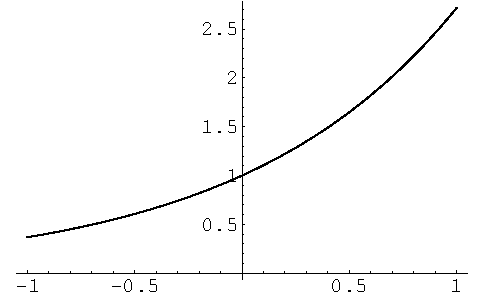
\includegraphics[width=4.0cm]{image4}}
%  \vspace{1.5cm}
  \centerline{(c) Result 4}\medskip
\end{minipage}
%
\caption{Example of placing a figure with experimental results.}
\label{fig:res}
%
\end{figure}


% To start a new column (but not a new page) and help balance the last-page
% column length use \vfill\pagebreak.
% -------------------------------------------------------------------------
%\vfill
%\pagebreak

\section{COPYRIGHT FORMS}
\label{sec:copyright}

You must include your fully completed, signed IEEE copyright release form when
form when you submit your paper. We {\bf must} have this form before your paper
can be published in the proceedings.

\section{REFERENCES}
\label{sec:ref}

List and number all bibliographical references at the end of the
paper. The references can be numbered in alphabetic order or in
order of appearance in the document. When referring to them in
the text, type the corresponding reference number in square
brackets as shown at the end of this sentence \cite{Jones2003}. An
additional final page (the fifth page, in most cases) is
allowed, but must contain only references to the prior
literature.

% References should be produced using the bibtex program from suitable
% BiBTeX files (here: strings, refs, manuals). The IEEEbib.bst bibliography
% style file from IEEE produces unsorted bibliography list.
% -------------------------------------------------------------------------
\bibliographystyle{IEEEbib}
\bibliography{literature}

\end{document}
